\documentclass[12pt,letterpaper]{article}
\usepackage[utf8]{inputenc}
\usepackage[spanish]{babel}
\usepackage{graphicx}
\usepackage[left=2cm,right=2cm,top=2cm,bottom=2cm]{geometry}
\usepackage{graphicx} % figuras
% \usepackage{subfigure} % subfiguras
\usepackage{float} % para usar [H]
\usepackage{amsmath}
%\usepackage{txfonts}
\usepackage{stackrel} 
\usepackage{multirow}
\usepackage{enumerate} % enumerados
\renewcommand{\labelitemi}{$-$}
\renewcommand{\labelitemii}{$\cdot$}
% \author{}
% \title{Caratula}
\begin{document}

% Fancy Header and Footer
% \usepackage{fancyhdr}
% \pagestyle{fancy}
% \cfoot{}
% \rfoot{\thepage}
%

% \usepackage[hidelinks]{hyperref} % CREA HYPERVINCULOS EN INDICE

% \author{}
\title{Caratula}

\begin{titlepage}
\begin{center}
\large{UNIVERSIDAD PRIVADA DE TACNA}\\
\vspace*{-0.025in}
\begin{figure}[htb]
\begin{center}

\includegraphics[width=7cm]{./images/logo}
\end{center}
\end{figure}
\vspace*{0.15in}
INGENIERIA DE SISTEMAS  \\

\vspace*{0.3in}
\begin{large}
\textbf{TITULO:} \\
\end{large}

\vspace*{0.1in}
\begin{Large}
\textbf{Informe de Laboratorio 05: AdventureWork} \\

\end{Large}

\vspace*{0.3in}
\begin{Large}
\textbf{CURSO:} \\
\end{Large}

\vspace*{0.1in}
\begin{large}
INTELIGENCIA DE NEGOCIOS\\
\end{large}

\vspace*{0.3in}
\begin{Large}
\textbf{DOCENTE:} \\
\end{Large}

\vspace*{0.1in}
\begin{large}
 Ing. Patrick Cuadros Quiroga\\
\end{large}

\vspace*{0.4in}
\vspace*{0.1in}
\begin{large}
\textbf{INTEGRANTES:} \\
\begin{flushleft}
Cespedes Medina, Christian Alexander \hfill	(2017057864)\\

\centering  %CENTRA UN TEXTO
\vspace*{0.9in}
\begin{large}
Tacna\\ 01-07-2019
\end{large}

\end{flushleft}
\end{large}
\end{center}

\end{titlepage}


\tableofcontents % INDICE
\thispagestyle{empty} % INDICE SIN NUMERO
\newpage
\setcounter{page}{1} % REINICIAR CONTADOR DE PAGINAS DESPUES DEL INDICE


\section{ACTVIVIDAD 01: Importación de Datos usando el Wizard - SQL MANAGMENT} 

1. Primeramente crearemos una base de datos llamada BDTEST.
	\begin{center}
	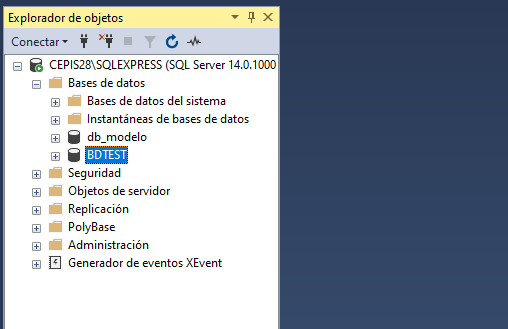
\includegraphics[width=\columnwidth]{images/task1/img1}
	\end{center}	


2. Ahora importaremos nuestra base de datos desde AdventureWorks.
	\begin{center}
	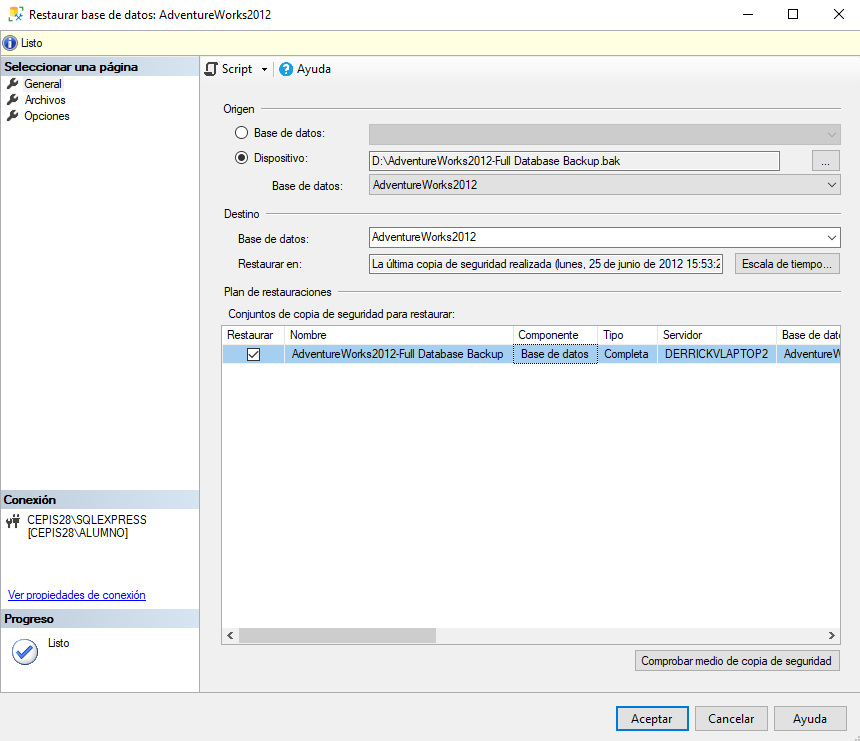
\includegraphics[width=\columnwidth]{images/task1/img2}
	\end{center}	

3. Next y escribir el Servidor y seleccionar la base de datosg.
	\begin{center}
	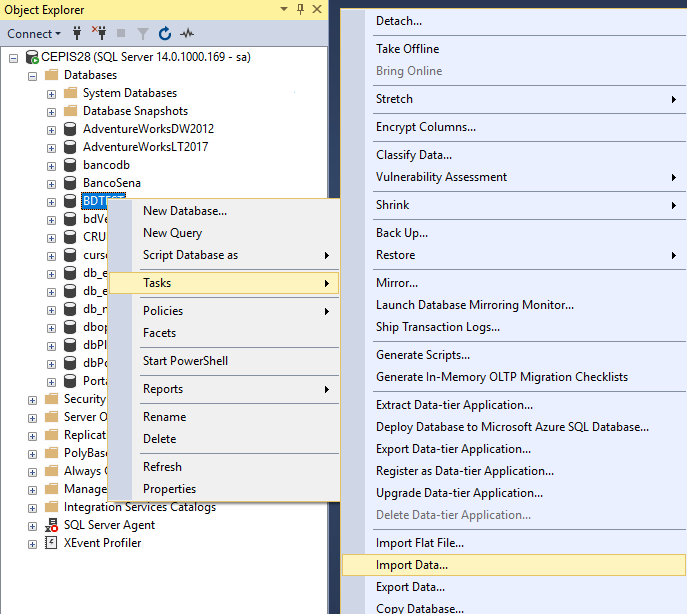
\includegraphics[width=\columnwidth]{images/task1/img3}
	\end{center}	

4. Data Source: La base de donde vamos a importar - Destination: La Base donde vamos a cargar la datas.
	\begin{center}
	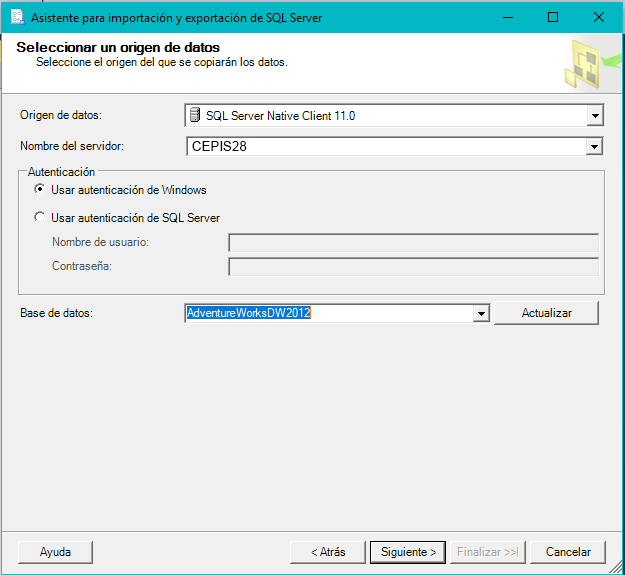
\includegraphics[width=\columnwidth]{images/task1/img4}
    \end{center}	
    
	\begin{center}
	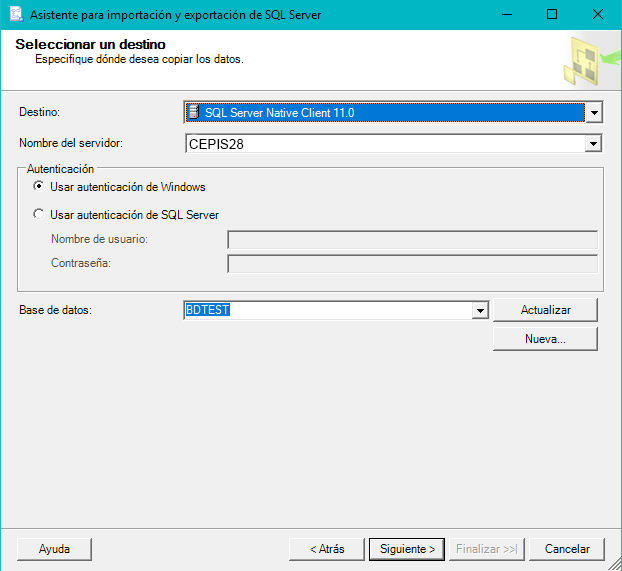
\includegraphics[width=\columnwidth]{images/task1/img5}
    \end{center}	
    
	\begin{center}
	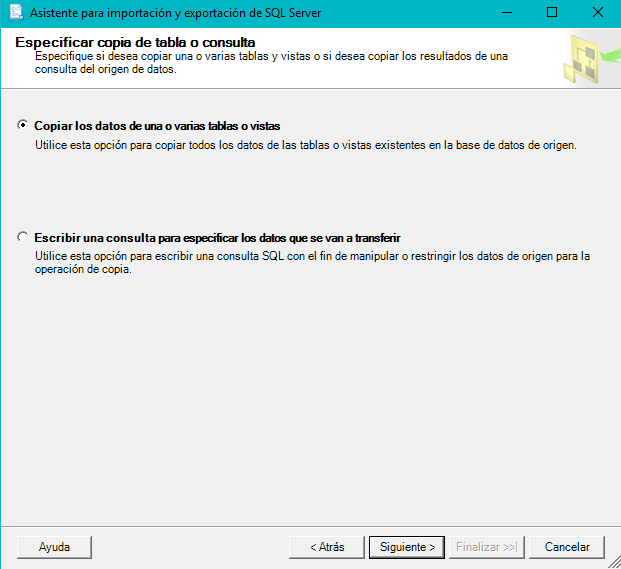
\includegraphics[width=\columnwidth]{images/task1/img6}
    \end{center}	
    
	\begin{center}
	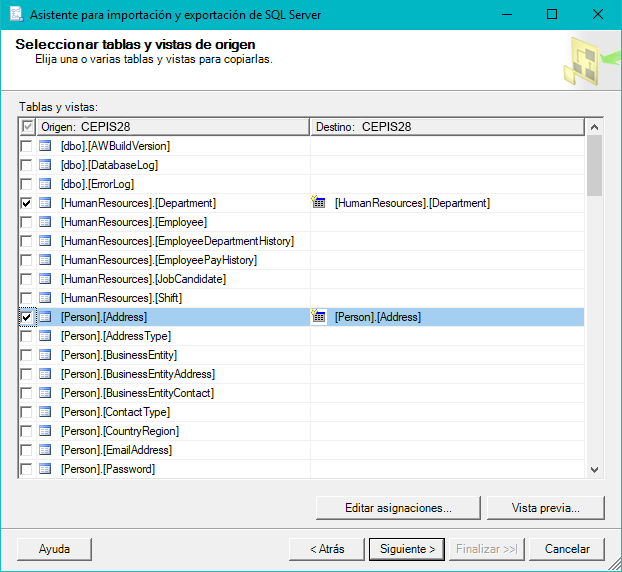
\includegraphics[width=\columnwidth]{images/task1/img7}
    \end{center}	
    
	\begin{center}
	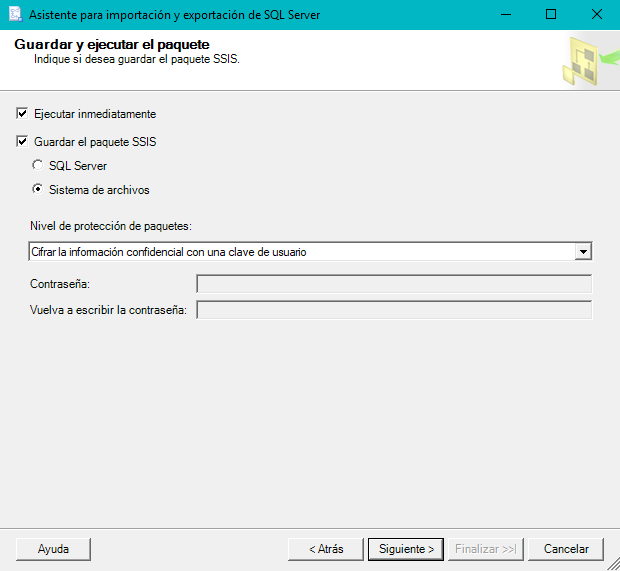
\includegraphics[width=\columnwidth]{images/task1/img8}
    \end{center}	
    
	\begin{center}
	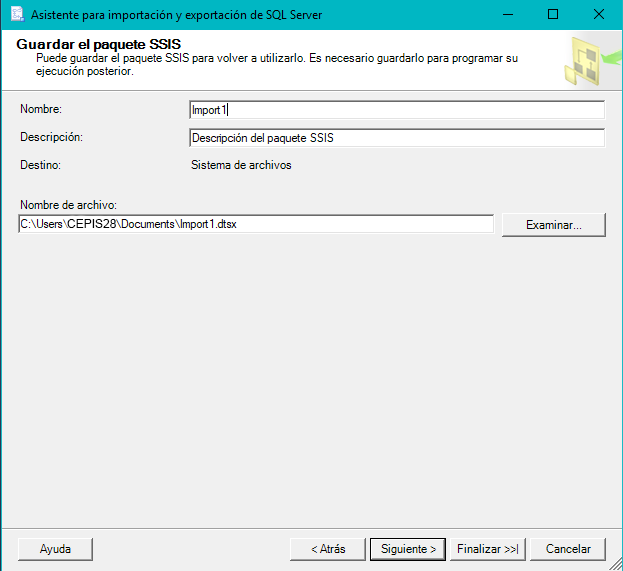
\includegraphics[width=\columnwidth]{images/task1/img9}
    \end{center}	
    
	\begin{center}
	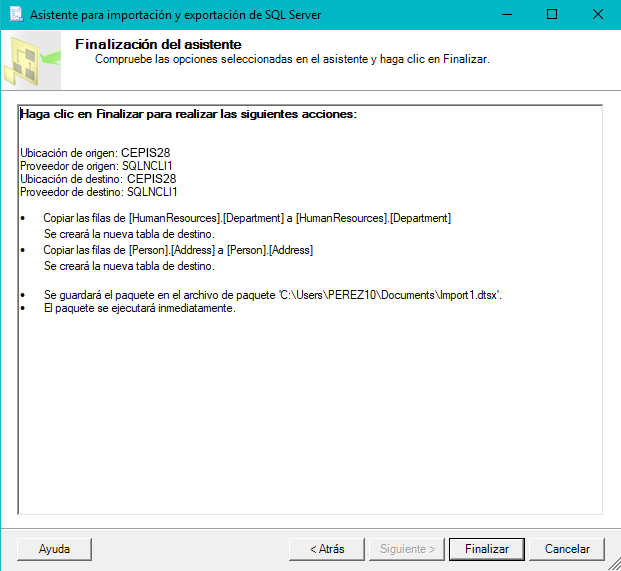
\includegraphics[width=\columnwidth]{images/task1/img10}
    \end{center}	
    
	\begin{center}
	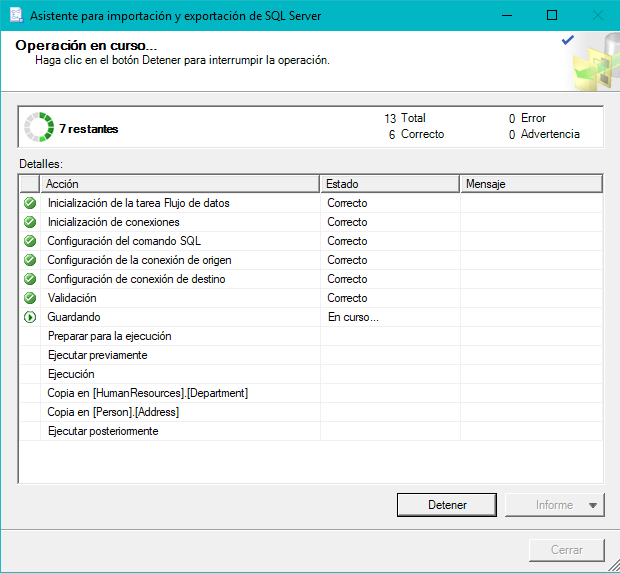
\includegraphics[width=\columnwidth]{images/task1/img11}
    \end{center}	
    
5. Al final veremos un resumen de la ejecución.
	\begin{center}
	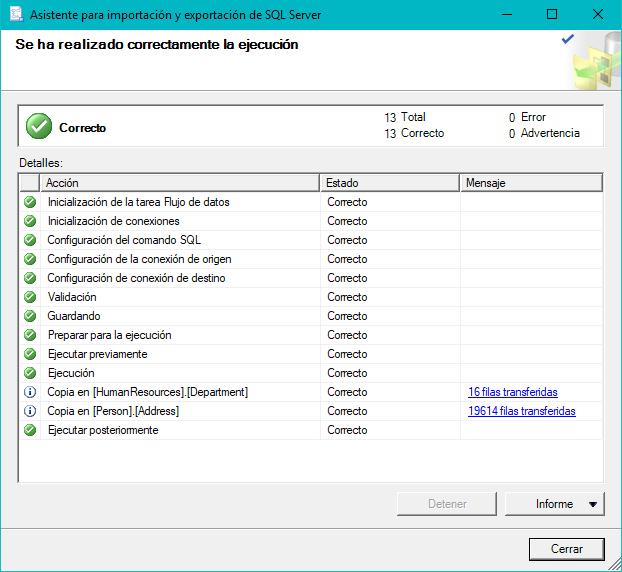
\includegraphics[width=\columnwidth]{images/task1/img12}
	\end{center}	
\section{ACTIVIDAD 02: Creación del primer paquete DTSX}

1. Abriremos un nuevo Proyecto en nuestro Visual Studio.
	\begin{center}
	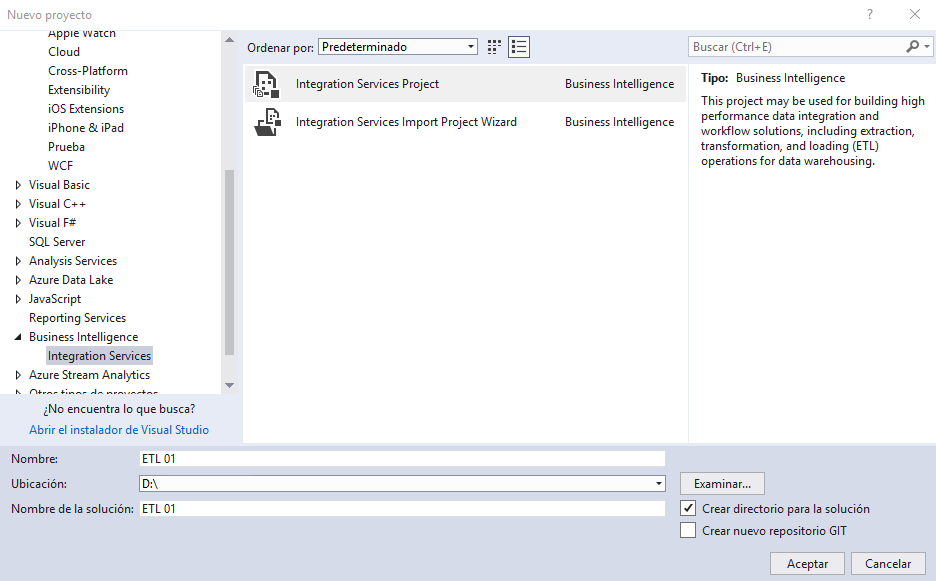
\includegraphics[width=\columnwidth]{images/task2/img13}
	\end{center}	

2. En al ventana nueva, sección Solución Explorer, Agrego el paquete generado antes.
	\begin{center}
	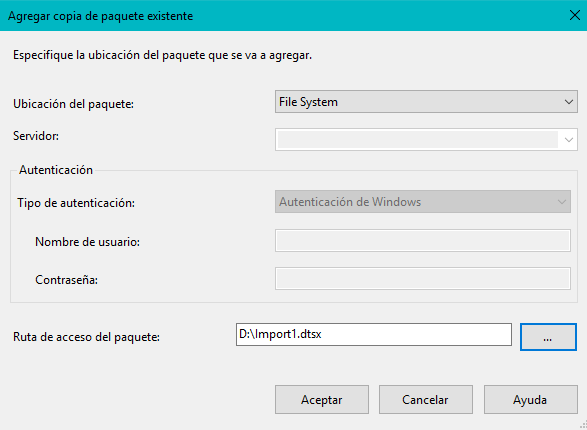
\includegraphics[width=\columnwidth]{images/task2/img14}
    \end{center}	
    
	\begin{center}
	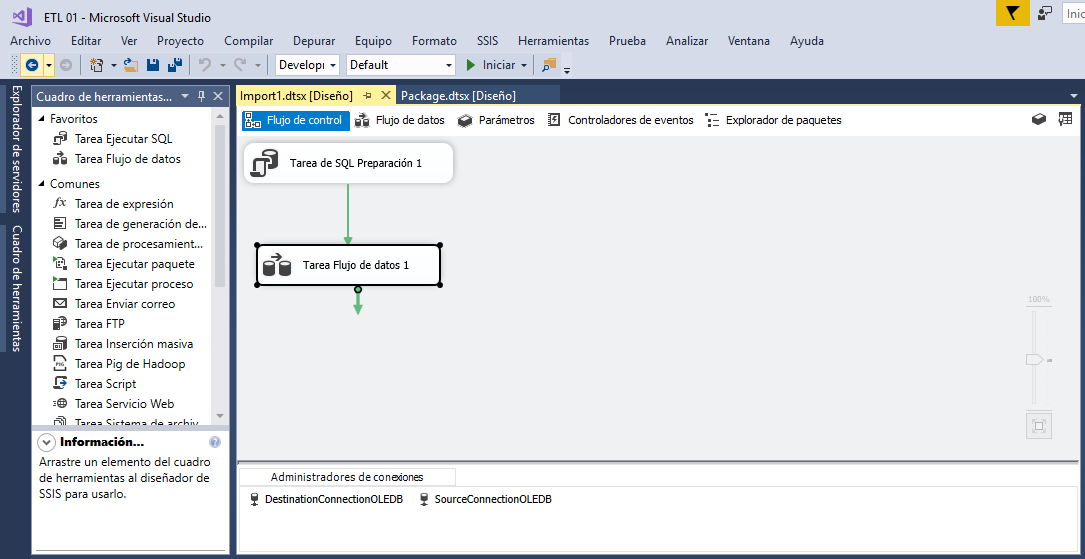
\includegraphics[width=\columnwidth]{images/task2/img15}
    \end{center}	
    
	\begin{center}
	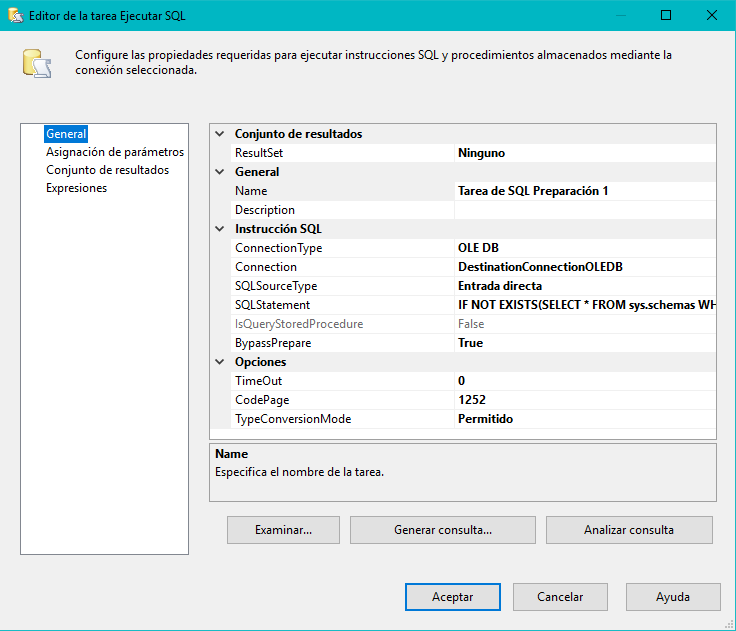
\includegraphics[width=\columnwidth]{images/task2/img16}
	\end{center}	

3. En la siguiente ventana mostramos el paquete que se ha importado.
	\begin{center}
	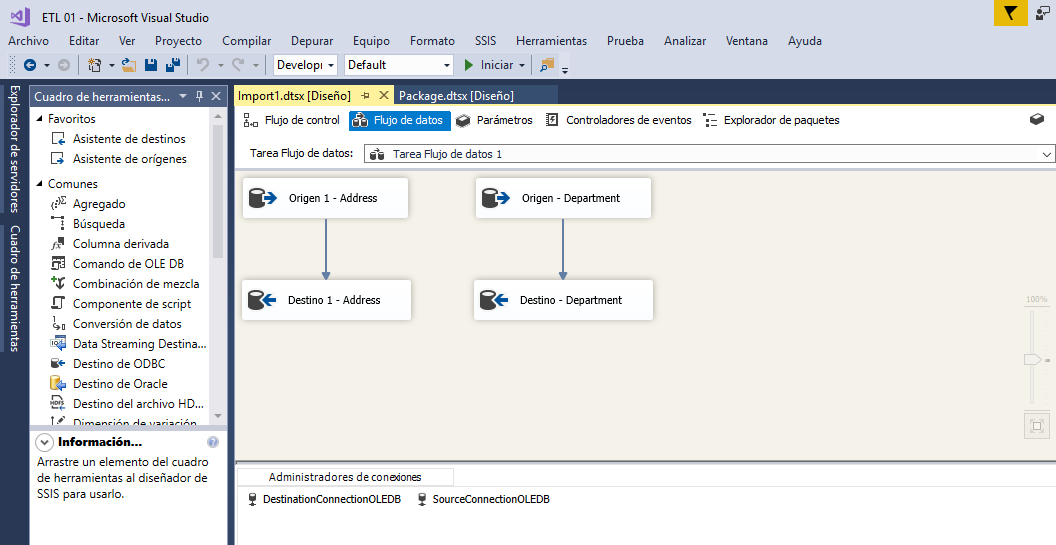
\includegraphics[width=\columnwidth]{images/task2/img17}
    \end{center}	
    
	\begin{center}
	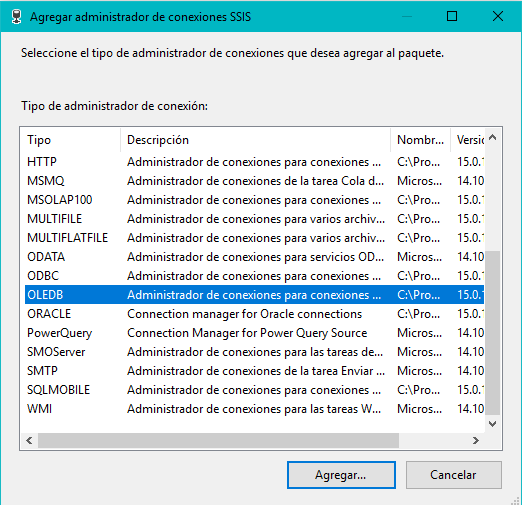
\includegraphics[width=\columnwidth]{images/task2/img18}
	\end{center}	

4. En la siguiente ventana mostramos el paquete que se ha importado.
	\begin{center}
	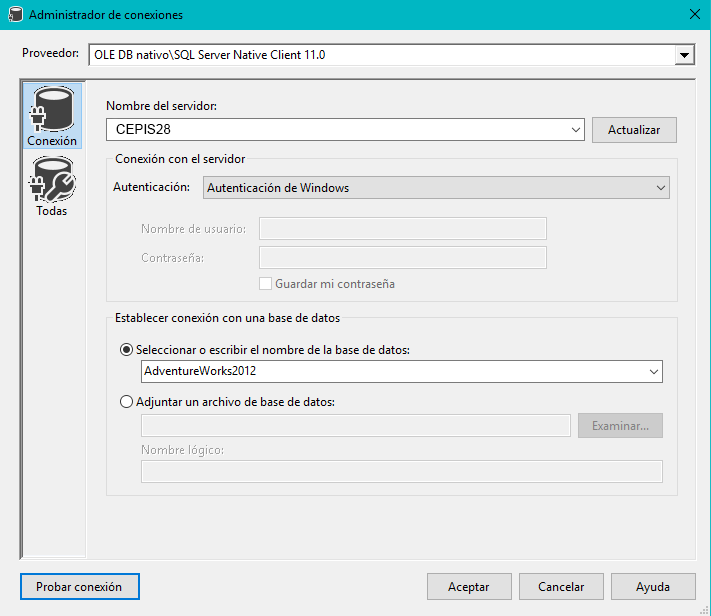
\includegraphics[width=\columnwidth]{images/task2/img19}
    \end{center}	
    
	\begin{center}
	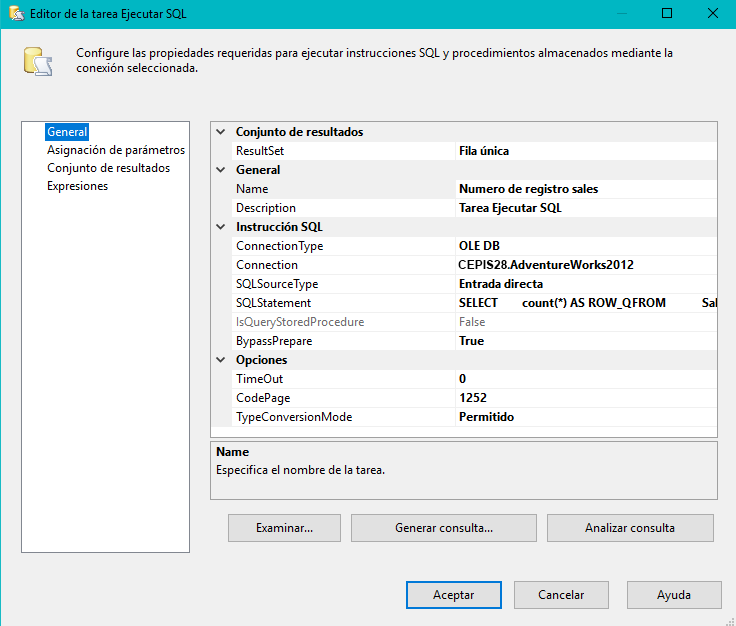
\includegraphics[width=\columnwidth]{images/task2/img20}
	\end{center}	
	

5. Editamos el componente Scrtipt Task Editor.
    \begin{center}
	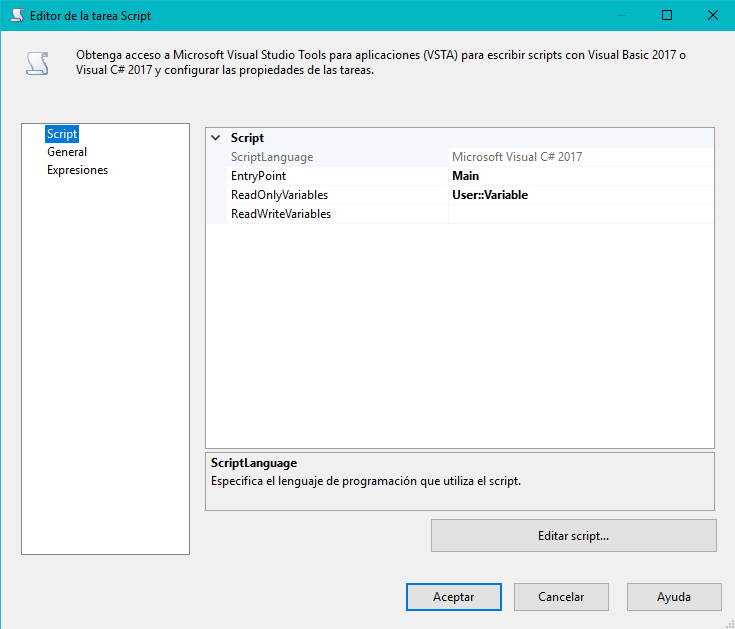
\includegraphics[width=\columnwidth]{images/task2/img21}
    \end{center}	
    
	\begin{center}
	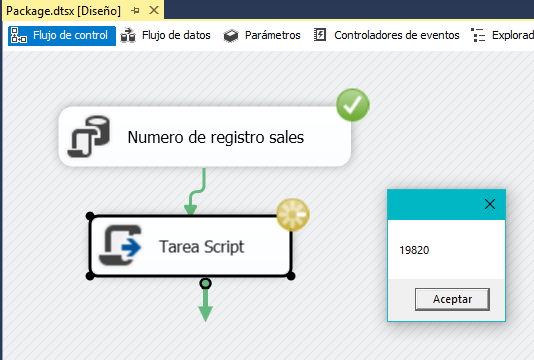
\includegraphics[width=\columnwidth]{images/task2/img22}
    \end{center}	
    
	\begin{center}
	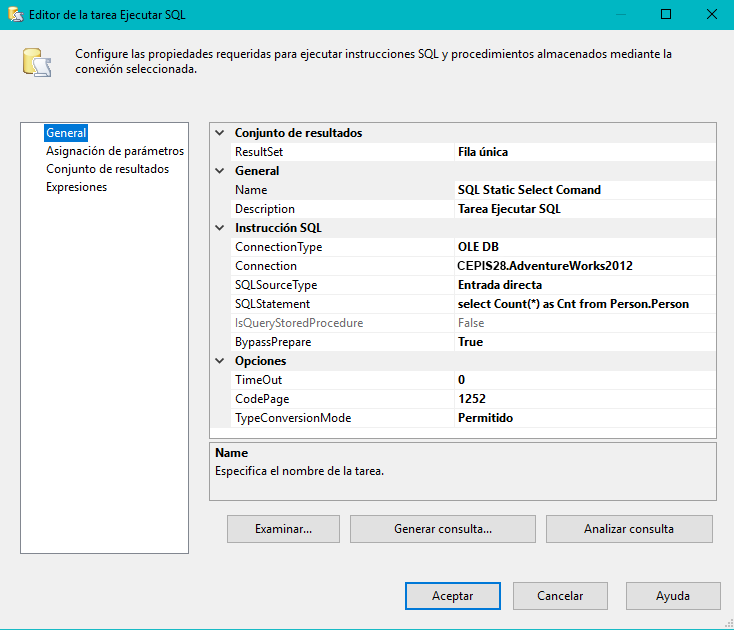
\includegraphics[width=\columnwidth]{images/task2/img23}
    \end{center}	
    
	\begin{center}
	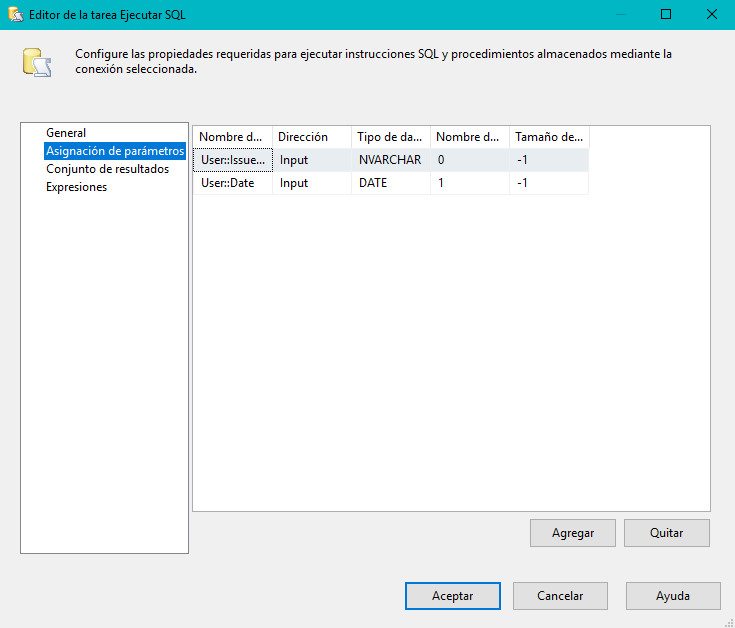
\includegraphics[width=\columnwidth]{images/task2/img24}
    \end{center}	
    
	\begin{center}
	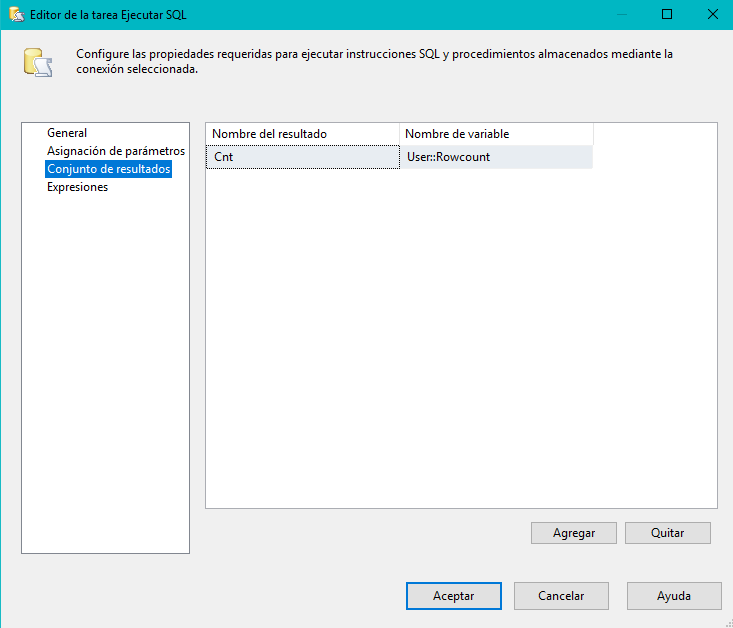
\includegraphics[width=\columnwidth]{images/task2/img25}
    \end{center}	
    
	\begin{center}
	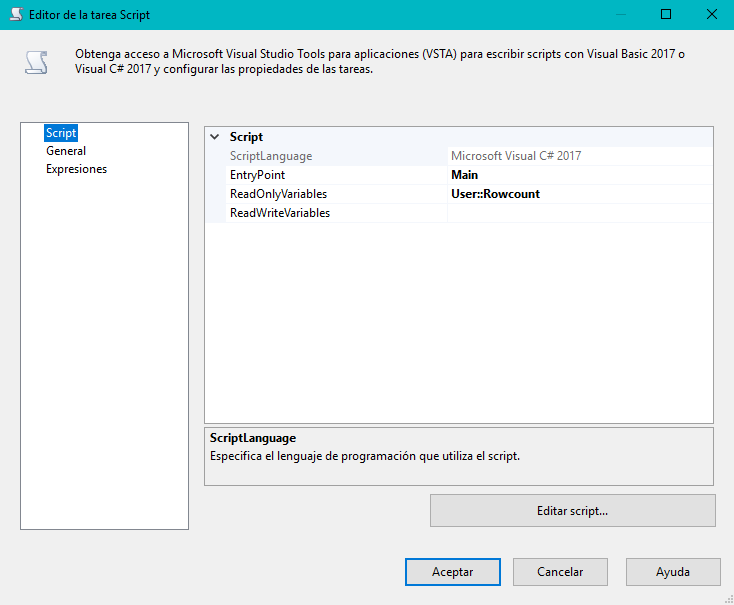
\includegraphics[width=\columnwidth]{images/task2/img26}
    \end{center}	

6. Guardamos y los ejecutamos.
    \begin{center}
	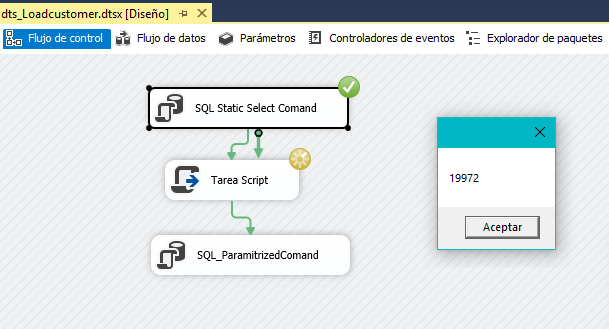
\includegraphics[width=\columnwidth]{images/task2/img27}
	\end{center}	

\end{document}